\section{Segmenter behaviour}

\subsection{VAD}

Whatever feature the VAD uses, it ultimately drives a state machine
with four states as illustrated in figure \ref{fig:StateMachine}.  The
purpose of the state machine is to place minimum time limits on speech
and silence segments.
\begin{figure}[htb]
  \centering
  \begin{tikzpicture}
    [inner sep=3mm,state/.style={circle,draw=black}]
    \node (silconf) at (0,2)  [state] {};
    \node (spetrig) at (2,0)  [state] {};
    \node (speconf) at (0,-2) [state] {};
    \node (siltrig) at (-2,0) [state] {};
    \node [above] at (silconf.north) {Silence Confirmed};
    \node [right] at (spetrig.east)  {Speech Triggered};
    \node [below] at (speconf.south) {Speech Confirmed};
    \node [left]  at (siltrig.west)  {Silence Triggered};
    \draw [->] (silconf) to [out=0,in=90]  (spetrig);
    \draw [->] (spetrig) to [out=-90,in=0] (speconf);
    \draw [->] (speconf) to [out=180,in=-90] (siltrig);
    \draw [->] (siltrig) to [out=90,in=180] (silconf);
    \draw [->] (spetrig) to [out=180,in=-90] (silconf);
    \draw [->] (siltrig) to [out=0,in=90] (speconf);
  \end{tikzpicture}
  \caption{VAD state machine}
  \label{fig:StateMachine}
\end{figure}

The state machine always begins in state ``Silence Confirmed'' and
moves to state ``Speech Triggered'' on voice activity.  If voice
activity remains for at least time $t_V$ then the state machine
progresses to state ``Speech confirmed'', otherwise it moves back to
``Silence Confirmed''.  A similar process governs the left hand half
of the state machine, depending on $t_S$, a time for silence
detection.  This is further illustrated in figure
\ref{fig:StateLevel}.
\begin{figure}[htb]
  \centering
  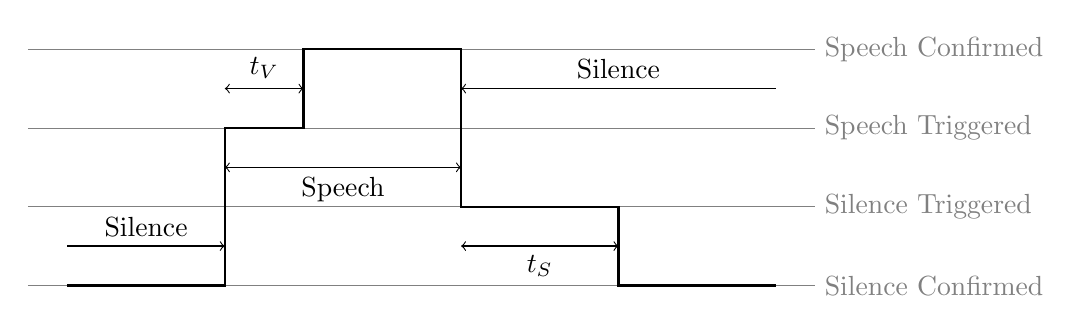
\begin{tikzpicture}
    \draw [help lines] (-.5,0) -- (9.5,0) node [right] {Silence Confirmed};
    \draw [help lines] (-.5,1) -- (9.5,1) node [right] {Silence Triggered};
    \draw [help lines] (-.5,2) -- (9.5,2) node [right] {Speech Triggered};
    \draw [help lines] (-.5,3) -- (9.5,3) node [right] {Speech Confirmed};
    \draw [thick] (0,0)
    -- (2,0)
    -- (2,2) -- (3,2)
    -- (3,3) -- (5,3)
    -- (5,1) -- (7,1)
    -- (7,0) -- (9,0);
    \draw [<->] (2,1.5) -- node [auto,swap] {Speech} (5,1.5);
    \draw [<->] (2,2.5) -- node [auto] {$t_V$} (3,2.5);
    \draw [<->] (5,0.5) -- node [auto,swap] {$t_S$} (7,0.5);
    \draw [->] (0,0.5) -- node [auto] {Silence} (2,0.5);
    \draw [<-] (5,2.5) -- node [auto] {Silence} (9,2.5);
  \end{tikzpicture}
  \caption{State level diagram for VAD.  Left to right dimension is
    time.}
  \label{fig:StateLevel}
\end{figure}


\subsection{Data flow}

Tracter components respond to fetch operations from the output caches.
The fetch will ask a component for a particular number of frames, $N$,
and the component should request enough data from its input components
to supply those $N$ frames.  The source components should block until
enough data become available.  The fetch operation should then return
an integer corresponding to the number of frames that were written to
the cache; this is normally $N$.

When data are no longer available, the components should return a
number less than $N$.  Such a case is always indicative of data flow
having been interrupted.  This is the only signal that a component is
able to send downstream to indicate that data is no longer available.
Call this the End Of Data signal (EOD).

Downstream components will typically simply pass on EOD by returning
frame counts less than those that were requested.  Some may choose to
take some ``edge effect'' action, duplicating the final frame for
instance, but will always eventually pass on EOD.

Depending upon the application, a sink component can restart data flow
by sending a reset signal.  This can be done, for instance, after
changing a file-name at the source.  Reset does not close connections;
it just resets counters and empties caches.

A (VAD) gate component is special because it can choose to block
reset.  When the end of a (speech) segment is detected, the gate
returns EOD.  The application then resets the flow graph and requests
more data.  Instead of propagating the reset upstream, the gate blocks
it and simply restarts data flow at the beginning of the next segment.
The gate component hence introduces extra EOD signals corresponding to
end of segment.  The application does not know the difference between
a real EOD and the fake EOD generated by the gate.

We have identified four different ``modes'' for the VAD gate in the
context of an application:
\begin{description}
\item[Offline] In offline mode, the input is typically a file.  The
  file is assumed to contain only one segment; the end of the segment
  is taken to be the end of the file.  The application resets after
  the segment; reset is likely to be accompanied by the application
  changing the file-name on the source.
\item[Offline segmented] As offline, but the file is assumed to
  contain several segments.  Reset should simply move to the next
  segment.  However, the end of the file is then difficult to spot.
  The VAD gate is aware of EOF because upstream components will
  indicate end of data.  The VAD gate indicates this to the
  application by returning 0 frames for the first fetch after the end
  of the file.  We call this a double EOD.
\item[Online] Online is taken to mean that the input is ``live'' in
  some sense.  The VAD gate is acting as a segmenter, and reset is
  taken to mean select the next segment.  The real end of data implies
  part of the system has shut-down.
\item[PTT] Push To Talk.  The data is online, but is being segmented
  to an extent by user intervention.  The end of data does not
  correspond to a shut-down; it just means that the application should
  wait until more data arrives.
\end{description}

\begin{table}[htb]
  \centering
  \begin{tabular}{|m{2cm}|m{3cm}|m{3cm}|m{3cm}|}
    \hline
    {\bf Mode} & {\bf Source} & {\bf Gate} & {\bf Sink / Application} \\
    \hline\hline
    Offline
    & EOD at EOF
    & Propagate reset
    & Reset after EOD, change file \\
    \hline
    Offline segmented
    & EOD at EOF
    & Block reset, propagate after EOD
    & Reset after EOD, change file after double EOD \\
    \hline
    Online
    & EOD at shut-down
    & Block reset
    & Shut-down after EOD \\
    \hline
    PTT
    & EOD at each segment
    & Propagate reset
    & Reset after EOD \\
    \hline
  \end{tabular}
  \caption{Mapping of segmentation modes to component behaviour.}
  \label{tab:SegmentationMode}
\end{table}

Table \ref{tab:SegmentationMode} shows the mapping between these modes
and behaviour of the source, gate and sink components.  Notice that:
\begin{enumerate}
\item The source really only has one mode: EOD is sent whenever it
  detects the end of a segment.
\item The gate has three modes, but given that the sink will never
  respond to a double EOD in online mode, it can be thought of as just
  two.  It doesn't care about whether it is online or offline, rather
  it needs to know whether to segment continuously or not.
\item The sink needs to be able to detect double EOD for the offline
  segmented mode.  However, given that it will only receive double EOD
  in that mode, it need not distinguish the special case.
\end{enumerate}


\subsection{Special cases}

The diagrams in figures \ref{fig:StateMachine} and
\ref{fig:StateLevel} are somewhat idealistic.  There are two
degenerate cases in particular that occur regularly, especially in
Offline and PTT modes:
\begin{enumerate}
\item No segment exists before EOF.
\item A segment begins but does not end before EOF.
\end{enumerate}
In the first case, the gate detects no signal at all and remains in
state ``Silence confirmed''.  In the second, the gate detects the
beginning of a signal, but not the end.


\subsection{Silence removal}

There is one more mode that is not mentioned above - Silence removal.
In this mode, silence between words is removed.  Without true
continuous speech recognition, this can only really work in cases
where there is another more persuasive utterance end indicator, i.e.,
the end of a file or a push-to-talk switch.




%%% Local Variables: 
%%% mode: latex
%%% TeX-master: "tracter"
%%% TeX-PDF-mode: t
%%% End: 
